%!TEX program = xelatex
%Template created by: Maciej Byczko
\documentclass[a4paper,12pt]{extarticle}  %typ dokumentu

\usepackage{geometry} %poprawienie marginesów
\usepackage{polski} %polskie znaki
\usepackage{graphicx} %grafiki
\usepackage{float} %poprawienie pozycji
\usepackage{fancyhdr} % header i footer
\usepackage{listings}
\usepackage{xcolor}
\usepackage{hyperref}
\graphicspath{{pictures/}}
\geometry{margin=0.7in}
\pagestyle{fancy}
\cfoot{Strona \thepage}
\rhead{Strona \thepage}
\lhead{\typdoc}
\setlength{\headheight}{15pt}

\title{\tytul \\ \small{\opis}}
\author{\tworcy}
\date{\data}

%-----------------------SEKCJA DANYCH----------------------------------
\def\tytul{Bluetooth - komunikacja z telefonem komórkowym} %<<< tytuł ćwiczenia
\def\nrcw{laboratoria 14} %<<< numer ćwiczenia
\def\data{\today} %<< data wykonania
\def\prowadzacy{Dr inż. Dominik Żelazny} %<<<prowadzący
\def\nrgrupy{D} %<<<numer grupy
\def\tworcy{Baraniecki Karol\\Byczko Maciej} %<<< autorzy
\def\zajinfo{PT 16:30 TP} %<<< informacje dotyczące zajęć
\def\typdoc{Sprawozdanie} %<<< typ dokumentu tj Sprawozdanie, zadania itp. {Matematyka dyskretna/Sprawozdanie z Miernictwa}
\def\opis{} %<<< opis który będzie umieszczony pod tytułem w Maketitle
%----------------------------------------------------------------------

\definecolor{backcolour}{rgb}{0.95,0.95,0.92}
\definecolor{AO}{rgb}{0,0.5,0}
\definecolor{ZeroBlue}{rgb}{0,0.28,0.73}
\definecolor{DarkRed}{rgb}{0.85,0.16,0.16}


\lstset{
basicstyle=\footnotesize,
breaklines=true,
language=Python,
numbers=left,
tabsize=2,
numberstyle=\tiny,
backgroundcolor=\color{backcolour},
breakatwhitespace=false,
showspaces=false,                
showstringspaces=false,
showtabs=false,
commentstyle=\color{gray},
keywordstyle=\color{ZeroBlue},
keepspaces=true,
% keywordstyle={[2]\color{DarkRed}},
% keywordstyle={[3]\color{ZeroBlue}},
}

\begin{document}
%-------------------------------------TABELA-DANYCH--------------------------------------------------
\begin{table}[H]
	\centering
	\resizebox{\textwidth}{!}{
		\begin{tabular}{|c|c|c|}\hline
			\begin{tabular}[c]{@{}c@{}}                     \tworcy     \end{tabular} &
			\begin{tabular}[c]{@{}c@{}}Prowadzący:\\        \prowadzacy \end{tabular} &
			\begin{tabular}[c]{@{}c@{}}Numer ćwiczenia\\    \nrcw       \end{tabular}          \\ \hline
			\begin{tabular}[c]{@{}c@{}}                     \zajinfo    \end{tabular} &
			\begin{tabular}[c]{@{}c@{}}Temat ćwiczenia:\\   \tytul      \end{tabular} & Ocena: \\ \hline
			\begin{tabular}[c]{@{}c@{}}Grupa:\\          \nrgrupy    \end{tabular}    &
			\begin{tabular}[c]{@{}c@{}}Data wykonania:\\    \data       \end{tabular} &        \\ \hline
		\end{tabular}}
\end{table}
%----------------------------------------------------------------------------------------------------
\section{Zagadnienia do opracowania}
% \subsection{Zasady korzystania z WinXP SP2 Api% SP2 (Service Pack 2) API - Niestety nigdzie nie mogliśmy znaleźć informacji na ten temat.
\subsection{MS Platform SDK}
zestaw do tworzenia oprogramowania (SDK) firmy Microsoft, który zawiera dokumentację, 
pliki nagłówkowe, biblioteki, próbki i narzędzia wymagane do tworzenia aplikacji dla systemu Microsoft Windows i .NET Framework.
Platform SDK specjalizuje się w tworzeniu aplikacji dla systemów Windows 2000, XP i Windows Server 2003.
Platform SDK jest następcą oryginalnego Microsoft Windows SDK dla Windows 3.1x i Microsoft Win32 SDK dla Windows 9x. 
Został wydany w 1999 roku i jest najstarszym SDK. 
Platform SDK zawiera kompilatory, narzędzia, dokumentacje, pliki nagłówkowe, biblioteki i próbki potrzebne do tworzenia oprogramowania na architekturach procesorów IA-32, x64 i IA-64. 

Zestawy SDK systemu Windows są dostępne za darmo; kiedyś były one dostępne w Centrum pobierania Microsoft, ale w 2012 roku zostały przeniesione do MSDN.

Programista może chcieć użyć starszego zestawu SDK z konkretnego powodu. Na przykład pakiet Windows Server 2003 Platform SDK wydany w lutym 2003 
roku był ostatnim pakietem SDK zapewniającym pełną obsługę Visual Studio 6.0. Niektóre starsze wersje PSDK można nadal pobrać z Centrum pobierania firmy Microsoft; 
inne można zamówić na płycie CD/DVD. 
\subsection{Znajomość funkcji}
Znajomość najważniejszych funkcji zdefiniowanych w:
\begin{enumerate}
	\item winsock2.h - najważniejsze funkcje:
	\begin{itemize}
		\item accept - zezwolenie na próbę połączenia przychodzącego na gniazdo.
		\item bind - skojarzenie adresu lokalnego z gniazdem.
		\item closesocket - zamknięcie istniejącego gniazda.
	\end{itemize}
	\item Ws2bth.h - najważniejsze interfejsy:
	\begin{itemize}
		\item BTH\_QUERY\_DEVICE - Wykorzystywana przy zapytaniu o obecność urządzenia Bluetooth.
		\item BTH\_QUERY\_SERVICE - Używana do odpytywania usługi Bluetooth.
		\item BTH\_SET\_SERVICE - Udostępnia informacje o usłudze dla określonej usługi Bluetooth.
		\item SOCKADDR\_BTH - Używana w połączeniu z operacjami na gniazdach Bluetooth, zdefiniowanymi przez rodzinę adresów AF\_BTH.
	\end{itemize}
	\item BluetoothAPIs.h - najważniejsze interfejsy:
	\begin{itemize}
		\item BluetoothGATTAbortReliableWrite - Określa koniec procedur niezawodnego zapisu, a zapisy powinny zostać przerwane.
		\item BluetoothGATTBeginReliableWrite - Informuje o rozpoczęciu niezawodnego zapisu.
		\item BluetoothGATTEndReliableWrite - Określa koniec niezawodnych zapisów, które powinny zostać wykonane.
		\item BluetoothGATTGetCharacteristics - Uzyskuje wszystkie charakterystyki dostępne dla określonej usługi.
		\item BluetoothGATTGetCharacteristicValue - Uzyskuje wartość określonej charakterystyki.
		\item BluetoothGATTGetDescriptors - Uzyskuje wszystkie deskryptory dostępne dla określonej charakterystyki.
		\item BluetoothGATTGetDescriptorValue - Uzyskuje wartość określonego deskryptora.
		\item BluetoothGATTGetIncludedServices - Uzyskuje wszystkie dołączone usługi dostępne dla danej usługi.
		\item BluetoothGATTGetServices - Pobiera wszystkie usługi podstawowe dostępne dla danego serwera.
		\item BluetoothGATTRegisterEvent - Rejestruje procedurę, która ma być wywoływana podczas zdarzenia zmiany wartości cechy na danej charakterystyce identyfikowanej przez jej uchwyt.
		\item BluetoothGATTSetCharacteristicValue - Zapisuje określoną wartość charakterystyki do urządzenia Bluetooth.
		\item BluetoothGATTSetDescriptorValue - Zapisuje określoną wartość deskryptora do urządzenia Bluetooth.
		\item BluetoothGATTUnregisterEvent - Wyrejestrowuje podane zdarzenie zmiany wartości charakterystyki.
	\end{itemize}
\end{enumerate}
\subsection{Ogólnie pojęcie o mechanizmach rejestracji funkcji callbackowych}
Wywołanie zwrotne (callback) - technika programowania będąca odwrotnością wywołania funkcji. Zwykle korzystanie z właściwości konkretnej biblioteki polega na wywołaniu funkcji (podprogramów) dostarczanych przez tę bibliotekę. W tym przypadku jest odwrotnie: użytkownik jedynie rejestruje funkcję do późniejszego wywołania, natomiast funkcje biblioteki wywołają ją w stosownym dla siebie czasie. 
\subsection{Zapoznanie się ze specyfikacją komunikacji poprzez BT}
Bluetooth jest otwartą specyfikacją standardu sieci, która umożliwia bezprzewodową, 
szybką komunikację na małe odległości między różnymi urządzeniami elektronicznymi (np. 
telefon komórkowy, PDA, piloty telewizyjne, laptopy, urządzenia peryferyjne) . Specyfikacja 
ta powstała, aby wyeliminować połączenia kablowe pomiędzy urządzeniami
\subsection{Protokół transferu plików OBEX}
OBEX (OBject EXchange [wymiana obiektów]) - protokół komunikacyjny, który ułatwia wymianę obiektów binarnych pomiędzy urządzeniami. 
Jest on utrzymywany przez Infrared Data Association, ale został również przyjęty przez Bluetooth Special Interest Group i skrzydło SyncML 
organizacji Open Mobile Alliance (OMA). Jednym z najwcześniejszych popularnych zastosowań OBEX był Palm III.
Ten PDA i jego liczni następcy używają OBEX do wymiany wizytówek, danych, a nawet aplikacji. Chociaż OBEX został początkowo zaprojektowany 
dla podczerwieni, obecnie został zaadoptowany przez Bluetooth, a także jest używany przez RS-232, USB, WAP oraz w urządzeniach takich 
jak smart-peny Livescribe. 

Znajomość poleceń:
\begin{itemize}
	\item CONNECT - Połącz
	\item PUT - Umieść
	\item DISCONNECT - Rozłącz
\end{itemize}
\section{Zadania do wykonania}
napisać aplikację graficzną, która:
\begin{enumerate}
	\item Wykryć adaptery BT podłączone do PC.
	\item Użyć wybranego adaptera do zdalnego wyszukiwania urządzeń BT.
	\item Pobrać adres MAC wybranego (wyszukanego w pkt. 2) urządzenia.
	\begin{figure}[H]
	   \centering
	   \resizebox*{\textwidth}{!}{
		  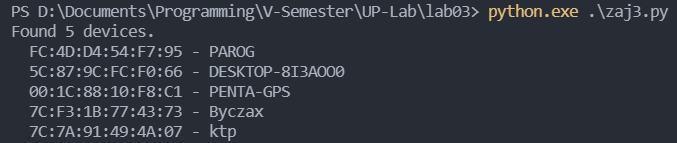
\includegraphics{discovered-devices.png}
	   }
	\end{figure}
	Nazwa naszego urządzenia to "Byczax"
	\item Dokonać autoryzacji obu urządzeń:
	      \begin{itemize}
		      \item po stronie urządzenia BT autoryzować PC
			  \begin{figure}[H]
				 \centering
				 \resizebox*{\textwidth}{!}{
					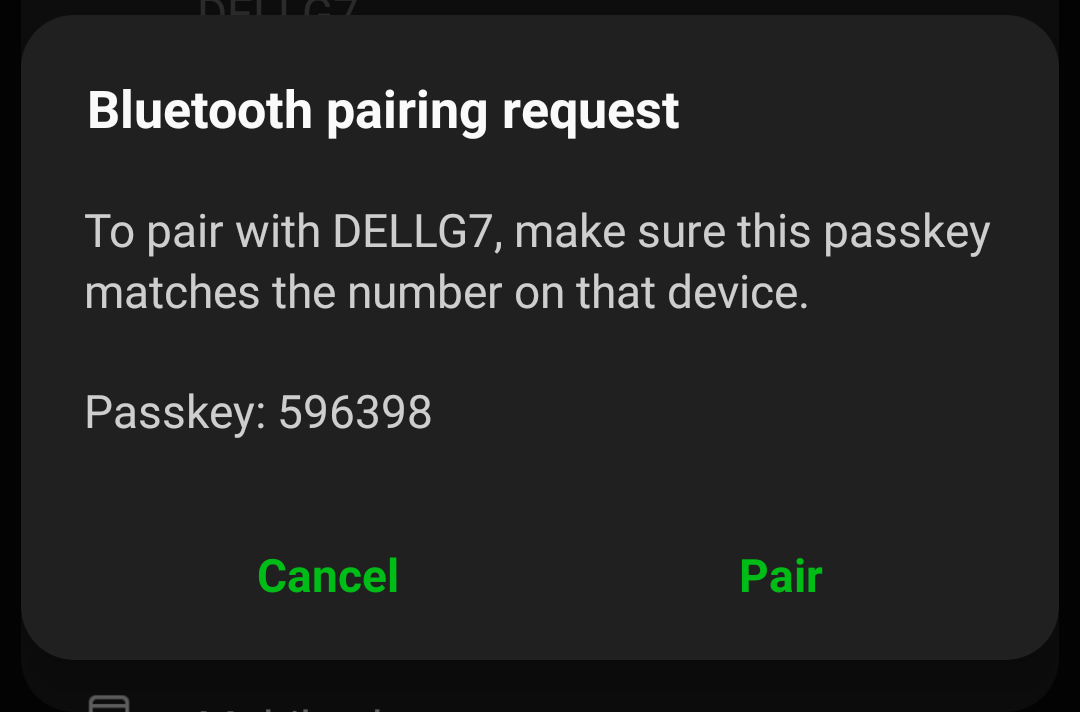
\includegraphics{connect-telefon.png}
				 }
			  \end{figure}
		      \item po stronie PC autoryzować urządzenie BT.
			  \begin{figure}[H]
				 \centering
				 \resizebox*{\textwidth}{!}{
					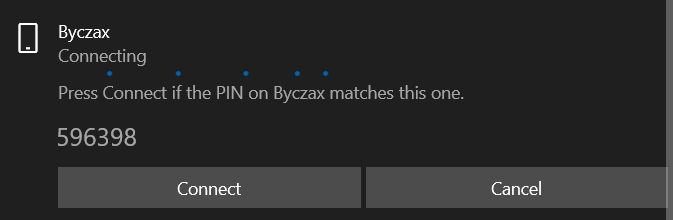
\includegraphics{connect-laptop.png}
				 }
			  \end{figure}
	      \end{itemize}
	\item Uruchomić urządzenie BT w tryb pracy transferu plików.
	\begin{lstlisting}
		karol@ktp ~/s5/UP/zaj3 % python3 all.py 7C:F3:1B:77:43:73
Found 12 services on 7C:F3:1B:77:43:73.

Service Name: None
    Host:        7C:F3:1B:77:43:73
    Description: None
    Provided By: None
    Protocol:    L2CAP
    channel/PSM: 31
    svc classes: ['1801']
    profiles:    []
    service id:  None

Service Name: None
    Host:        7C:F3:1B:77:43:73
    Description: None
    Provided By: None
    Protocol:    L2CAP
    channel/PSM: 31
    svc classes: ['1800']
    profiles:    []
    service id:  None

Service Name: Headset Gateway
    Host:        7C:F3:1B:77:43:73
    Description: None
    Provided By: None
    Protocol:    RFCOMM
    channel/PSM: 2
    svc classes: ['1112', '1203']
    profiles:    [('1108', 258)]
    service id:  None

Service Name: Handsfree Gateway
    Host:        7C:F3:1B:77:43:73
    Description: None
    Provided By: None
    Protocol:    RFCOMM
    channel/PSM: 3
    svc classes: ['111F', '1203']
    profiles:    [('111E', 262)]
    service id:  None

Service Name: AV Remote Control Target
    Host:        7C:F3:1B:77:43:73
    Description: None
    Provided By: None
    Protocol:    L2CAP
    channel/PSM: 23
    svc classes: ['110C']
    profiles:    [('110E', 259)]
    service id:  None

Service Name: Advanced Audio
    Host:        7C:F3:1B:77:43:73
    Description: None
    Provided By: None
    Protocol:    L2CAP
    channel/PSM: 25
    svc classes: ['110A']
    profiles:    [('110D', 259)]
    service id:  None

Service Name: None
    Host:        7C:F3:1B:77:43:73
    Description: None
    Provided By: None
    Protocol:    L2CAP
    channel/PSM: 23
    svc classes: ['110E', '110F']
    profiles:    [('110E', 261)]
    service id:  None

Service Name: Android Network Access Point
    Host:        7C:F3:1B:77:43:73
    Description: NAP
    Provided By: None
    Protocol:    L2CAP
    channel/PSM: 15
    svc classes: ['1116']
    profiles:    [('1116', 256)]
    service id:  None

Service Name: MAP SMS/MMS
    Host:        7C:F3:1B:77:43:73
    Description: None
    Provided By: None
    Protocol:    RFCOMM
    channel/PSM: 26
    svc classes: ['1132']
    profiles:    [('1134', 258)]
    service id:  None

Service Name: OBEX Phonebook Access Server
    Host:        7C:F3:1B:77:43:73
    Description: None
    Provided By: None
    Protocol:    RFCOMM
    channel/PSM: 19
    svc classes: ['112F']
    profiles:    [('1130', 258)]
    service id:  None

Service Name: SIM Access
    Host:        7C:F3:1B:77:43:73
    Description: None
    Provided By: None
    Protocol:    RFCOMM
    channel/PSM: 16
    svc classes: ['112D', '1204']
    profiles:    [('112D', 258)]
    service id:  None

Service Name: OBEX Object Push
    Host:        7C:F3:1B:77:43:73
    Description: None
    Provided By: None
    Protocol:    RFCOMM
    channel/PSM: 12
    svc classes: ['1105']
    profiles:    [('1105', 258)]
    service id:  None


	\end{lstlisting}
	\item Przesłać plik tekstowy do urządzenia BT.
	\begin{figure}[H]
	   \centering
	   \resizebox*{\textwidth}{!}{
		  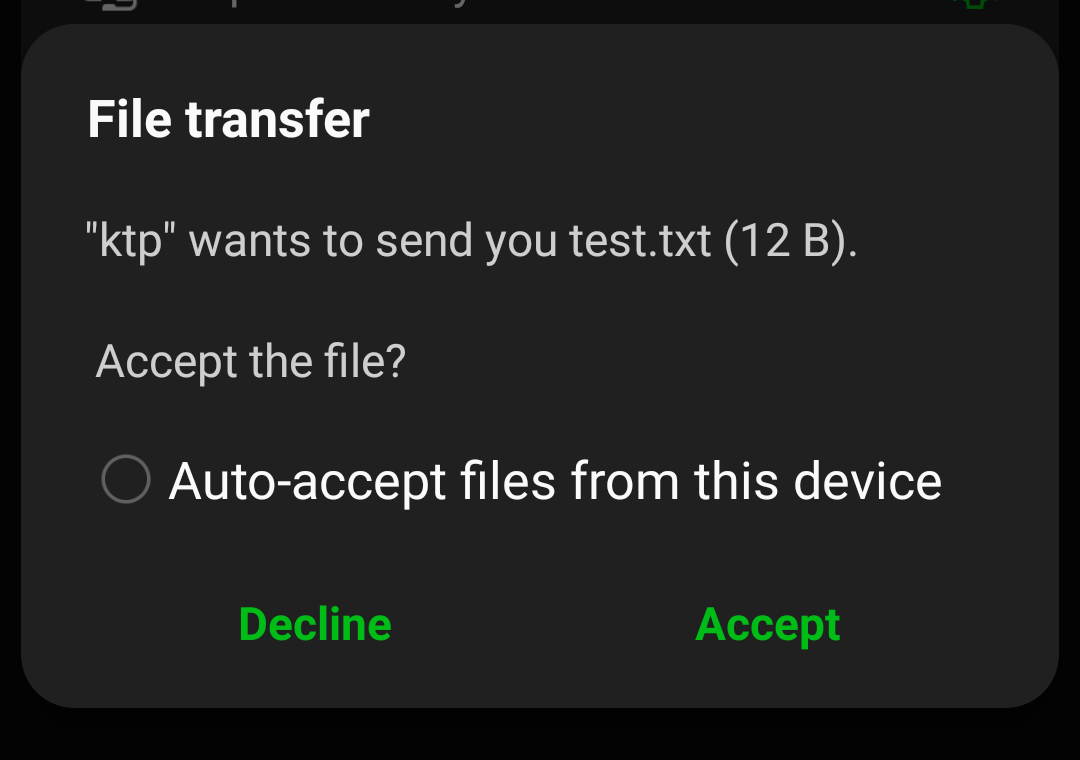
\includegraphics{send-text-file.png}
	   }
	\end{figure}
	\item Przesłać plik graficzny do urządzenia BT.
	\begin{figure}[H]
	   \centering
	   \resizebox*{\textwidth}{!}{
		  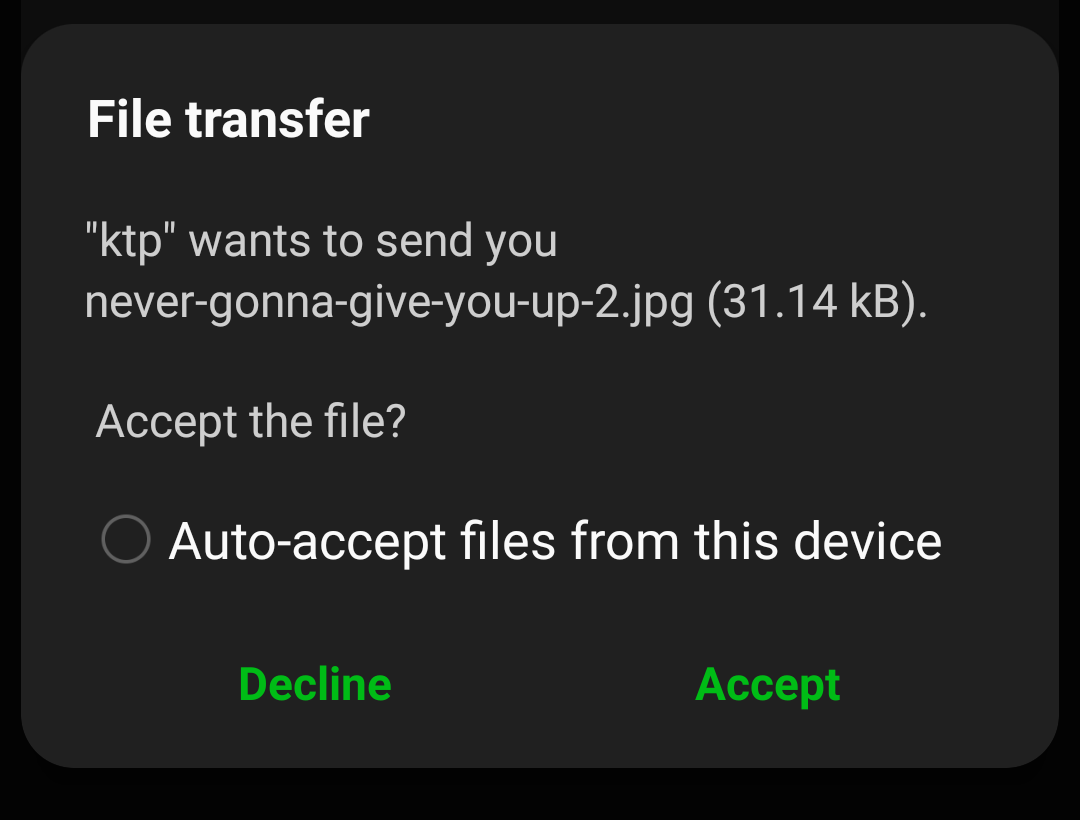
\includegraphics{sent-graphics-file.png}
	   }
	\end{figure}
\end{enumerate}
\section{Wnioski}
Bluetooth jest prosty w użyciu, wystarczyło zmienić rozszerzenie.
Cały kod został napisany w pythonie.\\
Problemy na które się natknęliśmy to:
\begin{itemize}
	\item Urządzenie wariowało gdy próbowało się podłączyć do kilku urządzeń,
	\item IPhone-y nie posiadają protokołu OBEX do przesyłania plików.
\end{itemize} 
\end{document}